\section{Aufgabe 2}
\label{sec:Aufgabe2}
\paragraph{a)}
Aufgrund der Symmetrie der Gauß-Kurve folgt 
\begin{equation}
g(x_j \vert x_i) = g(x_i \vert x_j) \implies \frac{g(x_j \vert x_i)}{g(x_i \vert x_j)} = 1 \; .
\end{equation}
Damit er gibt sich die Übergangswahrscheinlichkeit 
\begin{equation}
M_{i \rightarrow j} = \left(1 , \frac{f(x_j)}{f(x_i)} \frac{g(x_j \vert x_i)}{g(x_i \vert x_j)} \right) = \left(1 , \frac{f(x_j)}{f(x_i)} \right) = \text{Metroplolis-Algorithmus} \; .
\label{eq:Über}
\end{equation}
\paragraph{b)}
Der Algorithmus wurde als Funktion initialisiert, diese nimmt den Startwert, eine Anzahl an 
zu generierenden Werten, eine Schrittweite und eine Wahrscheinlickeitsverteilung entgegen.
Zuerst werden die Variablen \texttt{position, countDoku} und die Arrays \texttt{randoms,Iteration} 
definiert. Die Arrays werden nachher aufgefüllt und stellen die Rückgabe da. Die \texttt{position} 
stellt den aktuellen Wert des Algorithmus da. Die Variable \texttt{countDoku} dient hier als 
Zähler und gibt nachher den Iterationsschritt an, bei dem die Zufallszahl gezogen wurde, dieser 
wird im Array Iteration gespeichert. Beides ist Bestandteil des Aufgabenteils d). 
Die Variable \texttt{position} wird auf den Startwert gesetzt. Der Zähler natürlich auf Null. 
Nach der Definition folgt eine while-Schleife die erst beendet wird, wenn genügend Werte vom 
Algoritmus gezogen wurden. In der Schleife wird zuerst eine neue Zufallsvariable aus einer 
Gleichverteilung gezogen, diese stellt die zu überprüfende nächste Position da. 
Danach wird der Zähler erhöht.
Dann wird die Übergangswahrscheinlichkeit wie in \eqref{eq:Über} 
mit der übergebenen Wahrscheinlickeitsverteilung berechnet. Danach wird eine Zufallsvariable 
zwischen Null und Eins gezogen. Ist diese kleiner-gleich der Übergangswahrscheinlichkeit 
dann wird die aktuelle Position auf die nächste Position gesetzt und der Iterationsschritt 
(aktueller Wert des Zählers) gespeichert. Tritt der Fall ein, das die gezogene Zufallszahl größer 
ist als die Übergangswahrscheinlichkeit, wird ohne das etwas gespeichert wird wieder mit der 
Schleife begonnen.
\lstinputlisting[language=Python, firstline=11, lastline=28]{plots/Aufgabe2.py}
\paragraph{c)}
Die Planckverteilung wurde wie folgt initalisiert:
\lstinputlisting[language=Python, firstline=41, lastline=45]{plots/Aufgabe2.py}
\begin{figure}
  \centering
  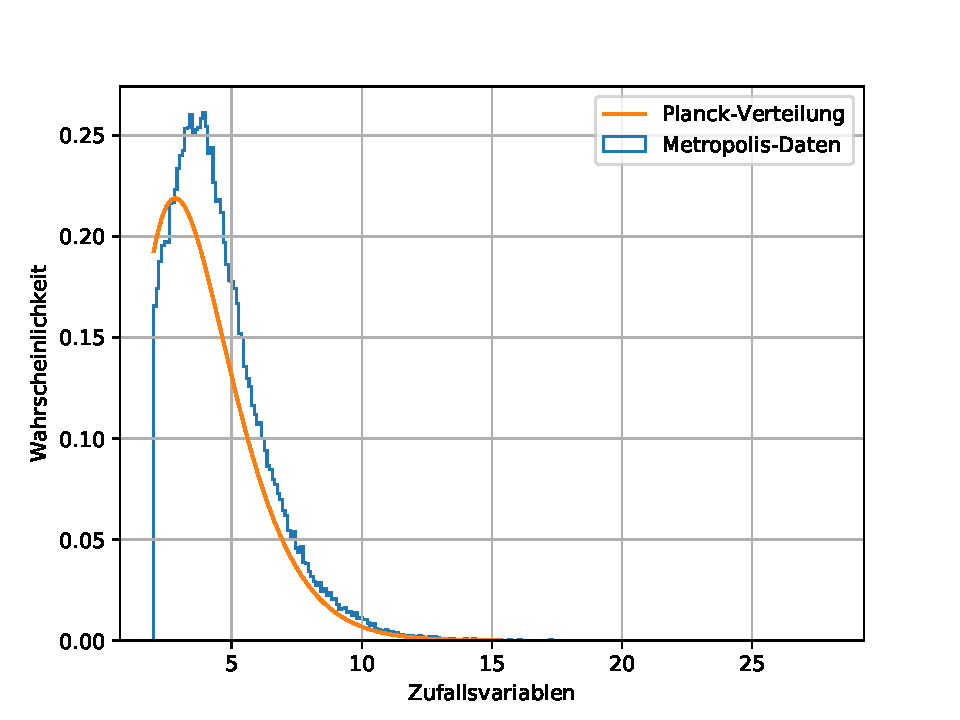
\includegraphics[height = 10cm]{plots/Planckvergleich.pdf}
  \caption{Gegenüberstellung der Daten des Metropolis Algorithmuses und der tatsächlichen Wahrscheinlickeitsverteilung.}
  \label{fig:Pvgl}
\end{figure}
Die Wahrscheinlickeitsverteilung und die dazugehörigen Daten aus dem Metroplolis 
Algorithmus mit Starwert 30 und Schrittweite zwei sind in Abbildung \ref{fig:Pvgl} gezeigt.
\paragraph{d)}
Das Traceplot ist in der Abbildung \ref{fig:Trace} dagestellt.
\begin{figure}
  \centering
  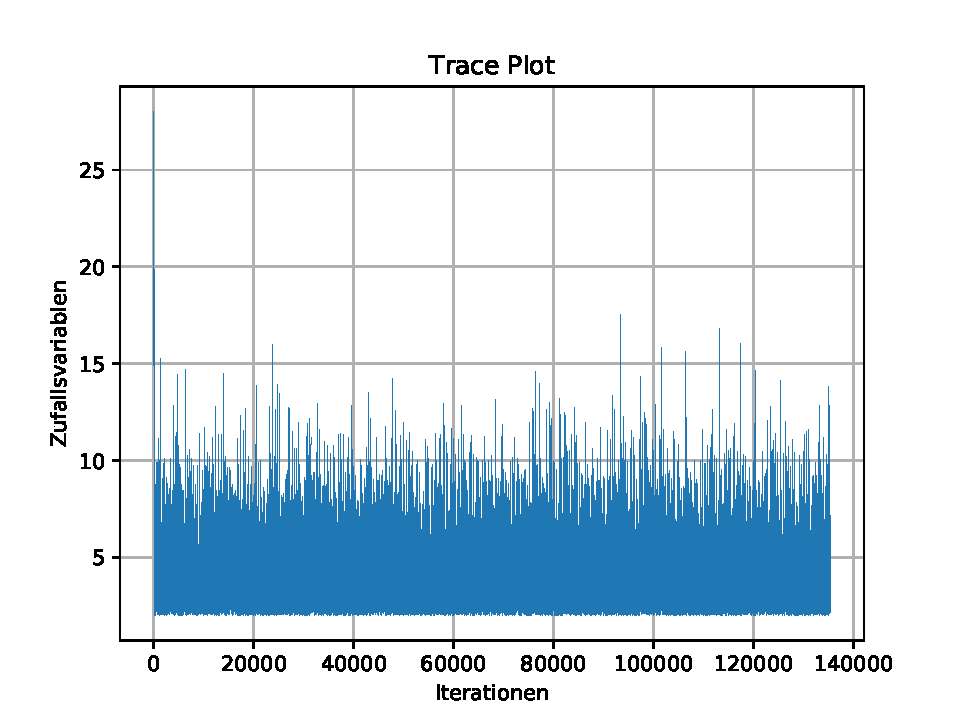
\includegraphics[height = 10cm]{plots/Traceplot.pdf}
  \caption{Traceplot für die Werte des Metroplolis Algorithmuses.}
  \label{fig:Trace}
\end{figure}

